%=========================================
\subsection{Video Search}
\label{videos}

VDMS provides full support for video storage and operations,
in a similar way it does for images.
This includes support for encoding, decoding, and transcoding of
\textit{mp4}, \textit{avi}, and \textit{mov} containers,
as well as support for \textit{xvid}, \textit{H.263} and \textit{H.264} encoders.
This is supported through the Visual Compute Module that provides an abstraction
layer on top of OpenCV~\cite{opencv} and \textit{libffmpeg}\cite{ffmpeg}.
All operations supported for images in VDMS are also supported at the
video and frame level of the API.
On top of that, there are a number of video-specific operations that
are supported, such as the interval operations,
enabling users to retrieve clips at different
frames-per-second (FPS) versions of the video.

We evaluate the performance and scalability of the video management
capabilities offered by VDMS.
Handling video in a general way is a complex task.
Some of this complexity comes from the existence of a variety of open and
proprietary implementations, different encoding techniques and container
formats, and different parameters of the video itself that are
application-dependent, like frames per second, lossy compression, etc.
When it comes to video, ad-hoc solutions have a large number of parameters that
can be tuned.
Together with that, there is no system that enables transactional
operations over videos files in the way VDMS does.
Because of this, we focus our efforts on understanding variations in the
performance of VDMS and its scalability, rather than comparing
it to a baseline that would not represent a fair
comparison for either of the systems.

\begin{figure*}[ht!]
\centering
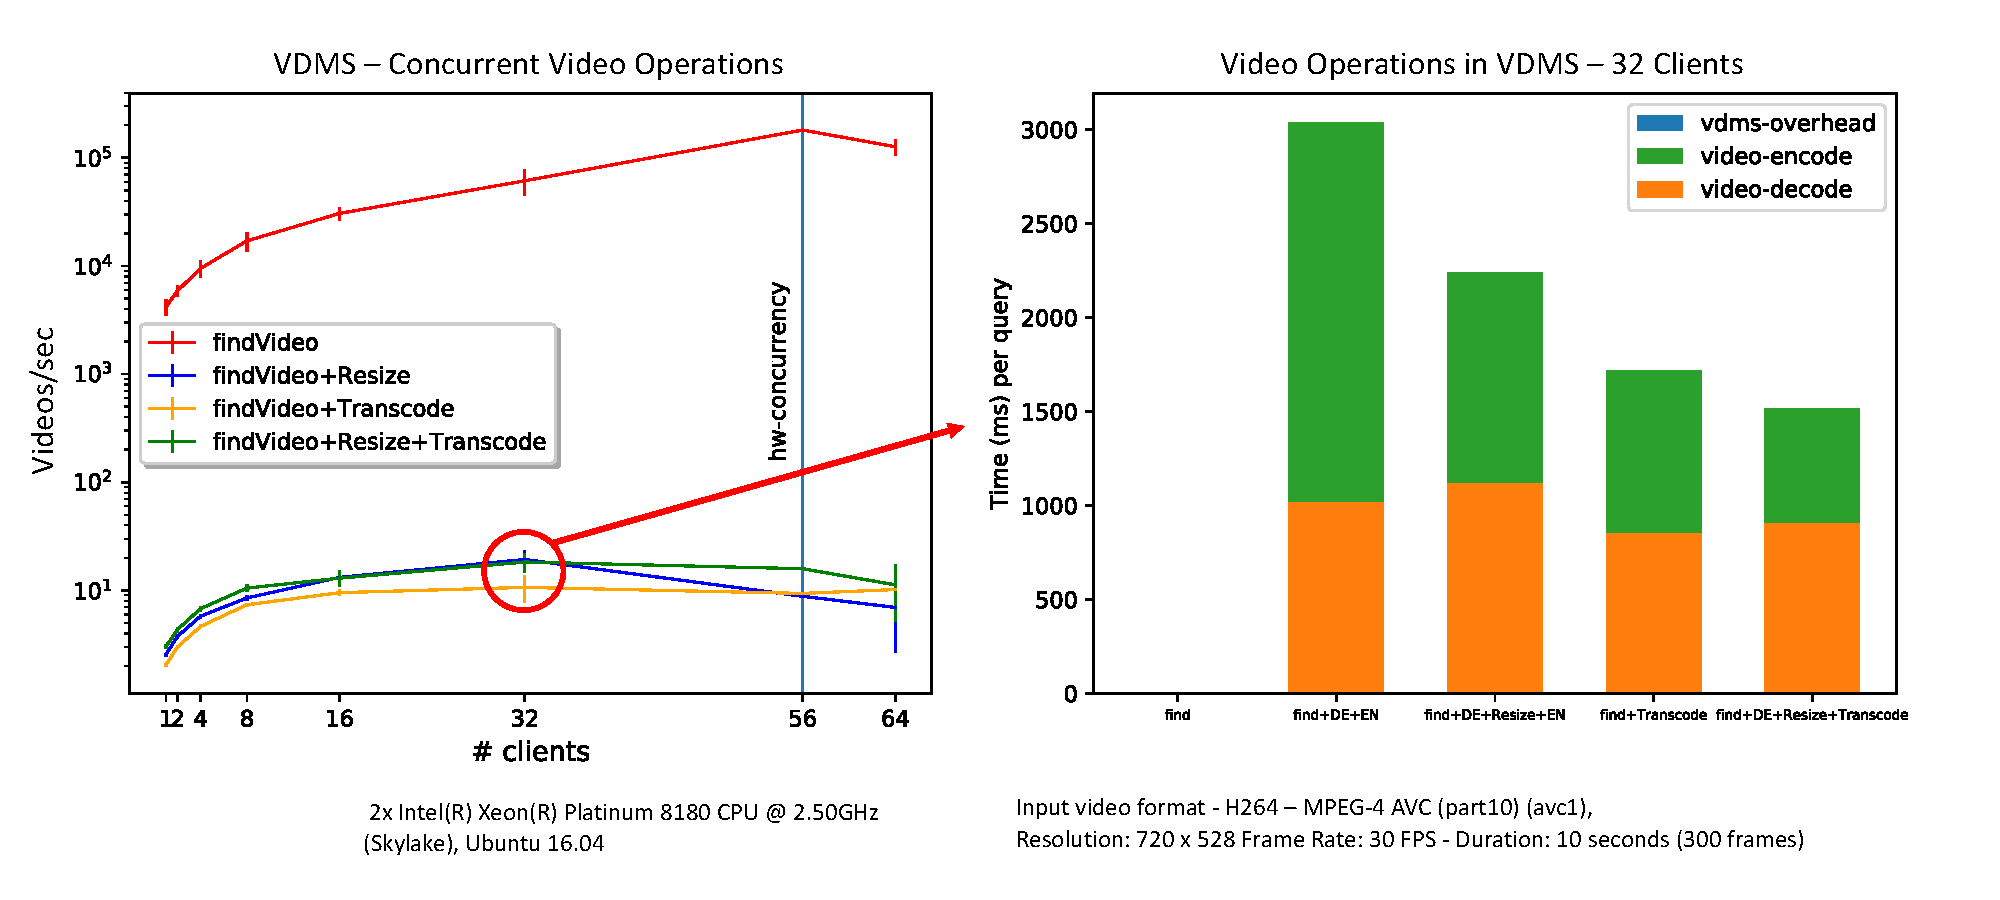
\includegraphics[width=\textwidth]{figures/video_overhead}
\caption{Analysis of video operations. The left figure shows the video throughput (videos per sec) as the number of concurrent clients increase and the right figure breaks down the different components of the
queries using 32 clients.}
\label{fig:video}
\end{figure*}

All this functionality is provided and integrated with the rest of the
metadata API as part of the comprehensive VDMS interface.
This makes it possible for users to interact with metadata and video in 
a transactional manner, enabling users to run queries like: 
"Retrieve all the videos where there is a \textit{lake} with 
probability higher than 0.86, converting all videos to \textit{H.264} 
\textit{mp4} of size 224x224".
Appendix shows a sample of how this query would be implemented using the VDMS API
\footnote{https://github.com/\{Not shown during submission\}}.
% \footnote{https://github.com/IntelLabs/vdms/wiki/FindVideo}.
In particular, this functionality was used internally to select a subset
of videos with the right licenses for a video summarization application.

To the best of our knowledge, there is no solution that can provide
all the functionality mentioned above, behind a single interface
that also allows users to interact with images and metadata.
Implementing a baseline, like we did for images, is significantly more complex
due to the parametrization of video encodings and containers, 
as explained at the beginning of this section.
For this reason, we chose to make a study using VDMS in various scenarios,
and analysis of scalability and the impact of having the overhead of VDMS' Request
Server in the overall access time and throughput.

Figure~\ref{fig:video} shows the analysis of different queries aimed
at retrieving a video using the VDMS interface.
We show how VDMS throughput increases when serving
a video object as the number of simultaneous clients increases, as well as the
overhead operations introduced in the overall query execution time.
The figure on the left compares the number of video transaction per second
(i.e., number of videos returned per second) when different operations
are executed as part of the transaction. The upper-bound of this would be
simply returning the video as-is (without running any encoding/decoding or
operation), represented by the red line. This query is the upper-limit because
it essentially translates to reading the video from the file-system and sending
it over a TCP/IP socket, without any other overhead or operations.

\begin{listing}[ht!]
\begin{minted}[frame=single,
               framesep=3mm,
               linenos=true,
               xleftmargin=21pt,
               tabsize=4]{js}
"FindEntity"{     
    "class": "autotag",
    "constraints": { 
        "name": ["==", "lake"]
    }
    "_ref" : 1
},
"FindVideo":{
    "container": "mp4",
    "codec": "h.264",
    "link": {
        "ref":1,
        "constraints": {
            "prob": [">=", 0.86]
        }
    }
    "operations": [{
        "type": "resize",
        "height": 1080,
        "width":  1920,
    }]
}

\end{minted}
\caption{Sample Query for Video - 
The query expresses the following: 
Find all videos connected to the autotag \textit{lake} 
with probability higher than 0.86, apply a resize operation
to make the video 1920×1080, and convert to "mp4" file, 
using H.264 encoding.} 
\label{findvideo}
\end{listing}

We also run a set of other queries that involve, showed in Figure~\ref{fig:video}:
(a) running a resize operation on the video and, consequently,
decoding and encoding operations as well (blue line),
(b) transcoding, meaning the use of a different container and encoder
than the one originally used (yellow line), and
(c) both resize and transcoding.
Note that the resize operation (blue and green lines) performs a downsize,
which translates in less data being sent over the wire.
This is specially noticeable when supporting 32 simultaneous clients, 
where the system provides more videos per second due to sending less data to 
the client, when compared to just transcoding and not resizing (yellow line).
We can see that the system performs best when using all the physical cores,
and this can be attributed to the compute-bound nature of video
encoding, decoding, and processing.

It is important to note an almost 3 orders of magnitude drop in performance
when including operations as part of the query.
We wanted to understand where most of the time was spent on the queries,
and optimize the Request Server and Visual Compute Module
if necessary. For this, we run the experiment shown at
Figure~\ref{fig:video} (right) which breaks down the different components of the
queries. This figure shows that more than 97\% of the query execution is spent
on encoding/decoding operations, which is well-known to be a
compute intensive operation\cite{videosgoogle}.
On the one hand, this result shows that VDMS barely introduces any overhead. 
On the other hand, this result means a limit on the opportunities 
for optimization for video queries given that biggest time factors 
are accounted by encoding/decoding, which is outside the scope of VDMS.
This result was the call to action for one optimization we will include
in future releases of VDMS, which involves using \textit{ffmpeg} C++ API to
limit the number of frames being encoded/decoded when possible.
This functionality will prevent encoding/decoding to happen on all frames
when users only need to retrieve a subset of the frames in the video.

%=========================================